\documentclass[a4paper,11pt]{article}
\usepackage[margin=23mm]{geometry}
\usepackage[T1]{fontenc}
\usepackage{lmodern}
\usepackage{amsmath,amssymb,bm,booktabs}
\usepackage{xcolor}
\usepackage{pgfplots}
\pgfplotsset{compat=1.18}
\usepackage[hidelinks]{hyperref}
\newcommand{\ii}{\mathrm{i}}
\newcommand{\Tr}{\operatorname{Tr}}
\newcommand{\ket}[1]{\lvert #1\rangle}
\newcommand{\bra}[1]{\langle #1\rvert}
\newcommand{\Diss}{\mathcal D}
\newcommand{\Ham}{\mathcal H}
\newcommand{\id}{\mathcal I}
\newcommand{\draftnote}[1]{\par\smallskip\noindent
  {\color{blue!55!black}\textbf{Draft status.} #1}\par\smallskip}
\setlength{\parskip}{0.25em}
\setlength{\parindent}{1em}
\allowdisplaybreaks

% Main manuscript from 2026-10-05 onward.
% Adopted claim: quantify Pauli-approximation errors after amplitude
% calibration in a finite-LD MS model with physical noise, and identify
% the components that dominate the discrepancy.
% Numerical provenance and unfinished validation: manuscript_notes.md.
% All plot coordinates and references are embedded for standalone compilation.

\title{Pauli-approximation errors after amplitude calibration\\
of thermally occupied M{\o}lmer--S{\o}rensen gates}
\author{}
\date{Working draft --- 5 October 2026}
\begin{document}
\maketitle
\draftnote{The numerical results below use saved simulation channels.
Final propagation convergence and comparison with the closest published
channel model remain to be completed. Appendix~\ref{sec:author_checks}
lists the checks required before submission.}

\begin{abstract}
Pauli noise models provide a compact description of imperfect entangling
gates, but their accuracy after calibration requires a channel-level
assessment. We study a two-ion, single-mode M{\o}lmer--S{\o}rensen gate
with a leading relative Lamb--Dicke correction and motional and spin
dissipation. Numerical process tomography is repeated after drive-amplitude
feedback that suppresses the coherent $XX$ angle error. We compare each
reduced error channel with its own Pauli twirl, using the diamond distance
and the structure of the discarded process-matrix elements. In the saved
data at mean phonon occupation $\bar n=4$, calibration reduces the
half-diamond distance from $7.41\times10^{-2}$ to $5.74\times10^{-3}$.
Across the five occupations studied, a real collective-$X$ cross-term
pattern accounts for $96.6$--$98.8\%$ of the squared off-diagonal
Frobenius norm after calibration. Its contribution also accounts for the
opposite discrepancies in two Bell-state survival probabilities.
These results quantify a residual error of the Pauli approximation
despite its exact preservation of average gate fidelity, and identify
the process-matrix components responsible within the studied model.
\end{abstract}

\section{Introduction}

Noise models used for trapped-ion quantum computation must describe both
the intended action of entangling gates and the errors that remain after
their calibration. A Pauli channel is convenient for simulating
stabilizer circuits, but replacing a physical channel by its Pauli twirl
discards information. In particular, the average gate fidelity is
unchanged by this replacement. A quantitative assessment therefore needs
an observable or channel distance that is sensitive to the omitted
terms. This issue becomes especially relevant after calibration removes
a large coherent error and exposes a smaller residual channel.

The physical effects of thermal motion on M{\o}lmer--S{\o}rensen (MS)
gates have an established theoretical basis. S{\o}rensen and
M{\o}lmer derived phonon-dependent coupling strengths beyond the
linear Lamb--Dicke approximation and showed that a correction to the
mean coupling leaves an error proportional to the phonon-number
variance~\cite{MS2000}. Conditional motional states also reduce spin
coherence when they fail to recombine; the dependence of this effect on
thermal occupation is incorporated in models of noisy global MS
interactions~\cite{Lotshaw2023}. Higher-order analyses provide
explicit error operators and corrections to drive amplitudes and pulse
shapes~\cite{Kirchhoff2025}. These results establish the mechanisms
and motivate a separate assessment of their reduced-channel
consequences after a specified calibration procedure.

Channel characterization itself is also well developed. Experimental
process tomography has resolved error-matrix signatures of power
miscalibration in MS gates~\cite{Tinkey2021}, while a general
error-generator framework separates Hamiltonian, stochastic, and
correlation components~\cite{Markovian_Errors}. Of particular
relevance here, Ma \textit{et al.} derived a reduced error channel for
motional dephasing whose Kraus operators contain a collective-spin
operator and its square; in the $X$ convention, the leading error
operator is proportional to $XI+IX$~\cite{Ma2025}. The existence of
this collective structure is thus established. Effective Pauli models
have also been constructed for multiqubit trapped-ion gates under
specified approximations and used for error-correction
simulations~\cite{Grossman2026}.

Here we assess the discrepancy introduced by the Pauli approximation
after drive-amplitude calibration, in a fixed single-mode MS model
that includes a relative $O(\eta^2)$ first-sideband correction and
several dissipative processes. We repeat the physical gate simulation
after calibration at each initial thermal occupation. This permits a
comparison of the channel before and after calibration while retaining
the accompanying change in nonunitary errors. We then quantify the
distance to the Pauli twirl and identify which discarded matrix
components dominate. Bell-state survival probabilities give a direct
interpretation of the discrepancy. The contribution sought is a
quantitative assessment of this approximation in the specified
calibrated setting; the thermal mechanisms and the collective
error operator provide the physical basis for interpreting the result.

\section{Methods}
\label{sec:methods}

We characterize the errors of a two-ion M{\o}lmer--S{\o}rensen (MS) gate
by reconstructing its reduced two-qubit channel from master-equation
simulations. The ideal gate is factored out before analyzing the process
matrix and its logarithmic error generator. We then calibrate the drive
amplitude, repeat the channel reconstruction, and compare the remaining
noise with its Pauli-twirled approximation. A separate calculation resolved
by the initial motional Fock state is used to identify the contribution of
thermal motion to the error structure.

\subsection{Effective spin--motion Hamiltonian}
\label{subsec:hamiltonian}

We consider two qubits coupled to a single collective motional mode.
Let $a$ and $a^\dagger$ be its ladder operators, $N=a^\dagger a$, and
$S_x=X\otimes I+I\otimes X$. With a fixed spin phase, the effective
interaction-picture Hamiltonian is
\begin{equation}
 H(t)=\hbar A(t)S_x\otimes
 \left[B e^{-\ii\Phi(t)}+B^\dagger e^{\ii\Phi(t)}\right],
 \qquad \Phi(t)=\int_0^t\delta(t')\,dt',
 \label{eq:methods_hamiltonian}
\end{equation}
where $A(t)$ is the effective sideband coupling in angular-frequency units
and $\delta(t)$ is the detuning from the motional sideband. The leading
Lamb--Dicke factor is already absorbed into $A(t)$. To retain the leading
relative correction to the first-sideband coupling, we use
\begin{equation}
 B=a-\frac{\eta^2}{2}(N+1)a
   =a\left(1-\frac{\eta^2}{2}N\right),
 \qquad
 B\ket{n}=\sqrt n\left(1-\frac{\eta^2 n}{2}\right)\ket{n-1},
 \label{eq:methods_B}
\end{equation}
where $\eta$ is the Lamb--Dicke parameter. Thus the model retains an
$O(\eta^2)$ correction relative to the linear force. It does not include
the full optical interaction to all orders or additional motional
sidebands. The leading-order reference model is obtained by setting
$B=a$ at the same effective coupling.

For the baseline rectangular pulse, $A(t)=A_0$ and $\delta(t)=\delta>0$,
with $T=2\pi/\delta$. In the leading-order model and in the absence of
dissipation, the motional trajectory closes at $T$, giving, up to a global
phase,
\begin{equation}
 U_{\mathrm{LD}}(T)=\exp(\ii\phi_{\mathrm{LD}}XX),
 \qquad \phi_{\mathrm{LD}}=4\pi(A_0/\delta)^2,
 \qquad XX=X\otimes X.
\end{equation}
We choose $A_0/\delta=1/4$ and define the target operation as
$U_\star=\exp(\ii\phi_\star XX)$ with $\phi_\star=\pi/4$.
All rotation-angle coefficients below use this convention, without a
factor of $1/2$ in the exponent.

\subsection{Initial state and dissipative dynamics}
\label{subsec:master_equation}

The spin and motion are initially uncorrelated. For each input spin state
$\rho$, we initialize the motion in a thermal state,
\begin{equation}
 \varrho(0)=\rho\otimes\rho_{\mathrm{th}}(\bar n),\qquad
 \rho_{\mathrm{th}}(\bar n)=\sum_{n=0}^{\infty}p_n\ket n\bra n,
 \qquad p_n=\frac{\bar n^n}{(1+\bar n)^{n+1}}.
 \label{eq:methods_thermal}
\end{equation}
The $\bar n=0$ case is understood as the motional ground state.
The joint density operator evolves according to
\begin{align}
 \dot\varrho={}&-\frac{\ii}{\hbar}[H(t),\varrho]
 +\Gamma_{\mathrm h}\bigl(\Diss[a]+\Diss[a^\dagger]\bigr)(\varrho)
 +\Gamma_{\mathrm m}\Diss[N](\varrho) \nonumber\\
 &+\sum_{j=1}^2\left[
 \left(\frac{\Gamma_{\mathrm s}}{2}+\Gamma_{\mathrm{Ray}}\right)
       \Diss[Z_j]
 +\frac{\Gamma_{\mathrm{Ram}}}{2}
       \bigl(\Diss[\sigma_j^+]+\Diss[\sigma_j^-]\bigr)
 \right](\varrho),
 \label{eq:methods_master}
\end{align}
where
\begin{equation}
 \Diss[L](\varrho)=L\varrho L^\dagger
   -\frac12\{L^\dagger L,\varrho\}.
\end{equation}
Identity operators on unaffected subsystems are implicit.
Here $\Gamma_{\mathrm h}$ describes motional diffusion, with
$d\langle N\rangle/dt=\Gamma_{\mathrm h}$ for this dissipator alone in
an untruncated oscillator; $\Gamma_{\mathrm m}$ describes motional
dephasing; and $\Gamma_{\mathrm s}=1/T_2^*$ describes independent spin
dephasing. Rayleigh and Raman scattering are represented by effective
two-level dephasing and symmetric spin-flip terms, respectively. Leakage
out of the qubit subspace is not included.

The initial occupation $\bar n$ and the dynamical noise rates are
independent model parameters. In particular, an initially thermal mode
does not imply that the heating terms describe equilibration with a bath
at the same temperature. The baseline comparison has no additional
quasi-static fluctuations of the drive amplitude, detuning, or spin phase.

\subsection{Channel reconstruction and removal of the ideal gate}
\label{subsec:channel_reconstruction}

We reconstruct the physical two-qubit channel
$\mathcal G(\rho)=\Tr_{\mathrm m}[\varrho(T)]$
using numerical quantum process tomography~\cite{QPT}. The input set
contains the 16 tensor products of the four single-qubit states
$\ket0\bra0$, $\ket1\bra1$, $\ket+\bra+$, and
$\ket{+\ii}\bra{+\ii}$, where
$\ket+=(\ket0+\ket1)/\sqrt2$ and
$\ket{+\ii}=(\ket0+\ii\ket1)/\sqrt2$.
The same initial thermal state and dynamical parameters are used for
every input. If $M_{\mathrm{in}}$ and $M_{\mathrm{out}}$ contain the
column-vectorized input and output density matrices, respectively, the
superoperator is $S_{\mathcal G}=M_{\mathrm{out}}M_{\mathrm{in}}^{-1}$.
This reconstruction uses the simulated density matrices directly and
does not include measurement sampling or state-preparation errors.

We define the post-gate noise channel by
\begin{equation}
 \mathcal E=\mathcal G\circ\mathcal U_\star^{-1},
 \qquad \mathcal G=\mathcal E\circ\mathcal U_\star,
 \qquad \mathcal U_\star(\rho)=U_\star\rho U_\star^\dagger.
 \label{eq:methods_postgate}
\end{equation}
Thus the noise is placed after the ideal gate. All subsequent error
matrices refer to $\mathcal E$, whose ideal limit is the identity channel.
Using the standard two-qubit Pauli operators
$P_\mu\in\{I,X,Y,Z\}^{\otimes2}$, ordered as
$II,IX,IY,IZ,XI,\ldots,ZZ$, we write
\begin{equation}
 \mathcal E(\rho)=\sum_{\mu,\nu=0}^{15}
       \chi_{\mu\nu}P_\mu\rho P_\nu^\dagger,
 \qquad
 R_{\mu\nu}=\frac14\Tr\!\left[P_\mu^\dagger\mathcal E(P_\nu)\right].
 \label{eq:methods_representations}
\end{equation}
Our normalization is $\Tr(P_\mu^\dagger P_\nu)=4\delta_{\mu\nu}$
and $\Tr\chi=1$ for a trace-preserving channel. Complete positivity and
trace preservation are checked using the Choi matrix
$J(\mathcal E)=\sum_{i,j}\ket i\bra j\otimes\mathcal E(\ket i\bra j)$,
which must satisfy $J\succeq0$ and $\Tr_{\mathrm{out}}J=I_4$.
Trace normalization of $\chi$ alone is not used as a physicality test.

For generator extraction and channel-distance calculations, we project
the reconstructed Choi matrix onto these two constraints in Frobenius
norm using Dykstra's alternating-projection algorithm. The unprojected
matrices are retained to assess the effect of this numerical correction.

\subsection{Error-generator decomposition}
\label{subsec:error_generator}

The effective error generator per gate is represented by the principal
matrix logarithm $K=\log R$. We record the imaginary remainder and the
reconstruction residual $\|e^K-R\|_F$. This finite-gate representation
does not assume that the reduced spin dynamics forms a time-homogeneous
Lindblad semigroup.

To distinguish Hamiltonian and non-Hamiltonian components, we use the
complete elementary-generator basis of Ref.~\cite{Markovian_Errors}.
For nonidentity Pauli operators $P,Q$, the convention is
\begin{align}
 \Ham_P(\rho)&=-\ii[P,\rho], &
 \mathcal S_P(\rho)&=P\rho P-\rho,\\
 \mathcal C_{P,Q}(\rho)&=P\rho Q+Q\rho P
            -\tfrac12\{PQ+QP,\rho\},\\
 \mathcal A_{P,Q}(\rho)&=\ii\left(P\rho Q-Q\rho P
            +\tfrac12\{[P,Q],\rho\}\right).
\end{align}
Their PTM representations span the 240-dimensional space of
trace-preserving, Hermiticity-preserving two-qubit generators. We obtain
the coefficients by linear least squares in
\begin{equation}
 \mathcal K=\sum_{P\ne II}h_P\Ham_P
     +\sum_{P\ne II}s_P\mathcal S_P
     +\sum_{P<Q}\left(c_{P,Q}\mathcal C_{P,Q}
                      +a_{P,Q}\mathcal A_{P,Q}\right).
 \label{eq:methods_full_generator}
\end{equation}
These are signed decomposition coefficients; they are not independently
constrained to be positive Lindblad rates.

We also examine a reduced three-component description,
\begin{equation}
 \mathcal K_3=h_{XX}\Ham_{XX}
           +\gamma_{XX}\Diss[XX]
           +\gamma_{\mathrm{col}}\Diss[S_x].
 \label{eq:methods_reduced_generator}
\end{equation}
The Hamiltonian contribution is obtained from the antisymmetric part of
$K$; the two dissipative coefficients are fitted to the remaining
symmetric part by nonnegative least squares. We report the reconstruction
residual rather than assuming that this reduced model exhausts the
channel. Its fitted $\gamma_{XX}$ and $\gamma_{\mathrm{col}}$ are
distinguished from the coefficients of the complete decomposition.
In particular,
$\Diss[S_x]=\mathcal S_{XI}+\mathcal S_{IX}+\mathcal C_{XI,IX}$,
so a collective $X$ contribution includes a cross term absent from a
model containing only independent $XI$ and $IX$ jumps.

\subsection{Drive-amplitude calibration}
\label{subsec:amplitude_calibration}

For amplitude feedback, the Hamiltonian coefficients are extracted by
least-squares projection of $(K-K^{\mathsf T})/2$ onto the Pauli
Hamiltonian generators. With our target-gate convention, a pure angle
error $U_{\mathrm{actual}}=\exp[\ii(\phi_\star-\epsilon)XX]$
gives $h_{XX}=\epsilon$; positive $h_{XX}$ therefore denotes
underrotation. Guided by the leading-order scaling
$\phi\propto A^2$, we update the rectangular-pulse amplitude as
\begin{equation}
 A_{k+1}=A_k
 \sqrt{\frac{\phi_\star}{\phi_\star-h_{XX}^{(k)}}}.
 \label{eq:methods_calibration}
\end{equation}
The update is used on the branch $\phi_\star-h_{XX}^{(k)}>0$.
After each update, the master equation and all 16 tomography inputs are
recomputed. Consequently, the calibrated channel includes changes in
both its coherent and nonunitary components. The quadratic relation is
an update estimate, not an exact expression for the corrected dynamics.

Calibration is performed independently at each $\bar n$, holding the
detuning, gate duration, and dissipative rates fixed. In particular, the
scattering rates are held fixed in this baseline comparison. The feedback
target is $|h_{XX}|<2\times10^{-3}$, with at most two updates in the
baseline protocol. The achieved residual is retained for every condition.
% AUTHOR CHECK: Keep the protocol aligned with the final figure dataset.
% The current five-point before/after data use one update at each nbar.

\subsection{Fock-state-resolved analysis of thermal errors}
\label{subsec:fock_analysis}

To isolate the Hamiltonian contribution of thermal motion, we set all
explicit dissipative rates to zero and replace the thermal initial state
by individual Fock states. Since $H(t)$ commutes with $S_x$, the unitary
propagator has the conditional form
\begin{equation}
 U(T)=\sum_{s\in\{-2,0,2\}}\Pi_s\otimes U_s(T),
 \qquad
 H_s(t)=\hbar sA(t)
   \left[B e^{-\ii\Phi(t)}+B^\dagger e^{\ii\Phi(t)}\right],
\end{equation}
where $\Pi_s$ projects onto a collective-spin eigenspace.
The $s=0$ branch is stationary in this interaction picture. We calculate
the overlap between the $s=2$ and $s=0$ motional branches,
\begin{equation}
 c_n=\bra n U_2(T)\ket n=r_n e^{2\ii\theta_n}.
 \label{eq:methods_fock_coherence}
\end{equation}
The phase, unwrapped across $n$, defines the effective Fock-conditioned
$XX$ angle $\theta_n$. The magnitude $r_n$ measures the loss of spin
coherence caused by distinguishable conditional motional states. For a
coherent superposition of the two spin branches and a pure Fock input,
$r_n<1$ signals residual spin--motion entanglement.

Using the thermal probabilities in Eq.~\eqref{eq:methods_thermal}, we
evaluate
\begin{align}
 \bar\theta&=\sum_n p_n\theta_n,
 &\sigma_\theta^2&=\sum_n p_n(\theta_n-\bar\theta)^2,\\
 Z&=\sum_n p_n e^{2\ii\theta_n},
 &C&=\sum_n p_n c_n.
\end{align}
The phase-only quantity $Z$ isolates angular dispersion, whereas $C$
also contains residual motional distinguishability. Useful diagnostics
are $h_{XX}^{\mathrm{Fock}}=\phi_\star-\tfrac12\arg C$ and
$\gamma_{\mathrm{phase}}=-\tfrac12\log|Z|$, with the angular branch
chosen continuously near the target. For a narrow angular distribution,
$\gamma_{\mathrm{phase}}\simeq\sigma_\theta^2$.
These diagnostics are compared with the reconstructed generators; a
single branch overlap is not assumed to determine the entire two-qubit
channel. In particular, a collective dissipative interpretation is
assessed using the complete generator and the residual of
Eq.~\eqref{eq:methods_reduced_generator}.

\subsection{Comparison with the Pauli-twirled channel}
\label{subsec:pauli_comparison}

For each channel before and after calibration, we construct its own
Pauli-twirled approximation,
\begin{equation}
 \mathcal T(\mathcal E)(\rho)
 =\frac1{16}\sum_{P\in\{I,X,Y,Z\}^{\otimes2}}
   P^\dagger\mathcal E(P\rho P^\dagger)P
 =\sum_\mu\chi_{\mu\mu}P_\mu\rho P_\mu^\dagger.
 \label{eq:methods_twirl}
\end{equation}
Thus $\chi_{\mathrm P}=\operatorname{diag}(\chi)$ and
$R_{\mathrm P}=\operatorname{diag}(R)$. Twirling is applied to the
channel, not to its logarithmic generator. The average gate infidelity
relative to $U_\star$ is
\begin{equation}
 r=1-F_{\mathrm{avg}}(\mathcal G,\mathcal U_\star)
   =\frac45(1-\chi_{II,II}).
\end{equation}
It is unchanged by Pauli twirling and therefore cannot quantify the
accuracy of that approximation.

We instead evaluate the diamond distance
\begin{equation}
 \epsilon_{\mathrm P}
   =\frac12\|\mathcal E-\mathcal T(\mathcal E)\|_\diamond,
 \label{eq:methods_diamond}
\end{equation}
using primal and dual semidefinite programs~\cite{WatrousDiamond} and
retaining their numerical bounds and gap. As complementary diagnostics,
we report
\begin{equation}
 D_F=\|R-R_{\mathrm P}\|_F,\qquad
 f_F=\frac{D_F}{\|R-I_{16}\|_F},\qquad
 D_J=\frac12\left\|\frac{J(\mathcal E)-J(\mathcal T(\mathcal E))}{4}
        \right\|_1.
 \label{eq:methods_distances}
\end{equation}
Here $\|\cdot\|_1$ is the trace norm and $f_F$ is undefined for the
identity channel. These distances describe the error in replacing a
single physical channel by its Pauli approximation. Logical error rates
of a particular QEC circuit are not computed in this analysis.

\subsection{Numerical settings}
\label{subsec:numerics}

The baseline parameters are listed in Table~\ref{tab:methods_parameters}.
The current before/after channel comparison uses
$\bar n\in\{0.01,1,2,3,4\}$. The equations are integrated with QuTiP,
using absolute and relative solver tolerances of $10^{-12}$ and
$10^{-9}$. Time-dependent Hamiltonian coefficients are sampled at 500
uniformly spaced times over the gate and linearly interpolated; this
coefficient grid is distinct from the adaptive integration steps.
The simulation uses dimensionless values $A_0=0.125$, $\delta=0.5$, and
$T_{\mathrm{sim}}=4\pi$. Physical dissipative rates are multiplied by
$T/T_{\mathrm{sim}}$ when expressed in these simulation units.

\begin{table}[htbp]
 \centering
 \caption{Baseline physical parameters. $A_0$ denotes the effective
 sideband coupling defined in Eq.~\eqref{eq:methods_hamiltonian}.}
 \label{tab:methods_parameters}
 \begin{tabular}{ll}
  \toprule
  Parameter & Value\\
  \midrule
  Gate duration $T$ & $100\,\mu\mathrm{s}$\\
  Detuning $\delta/(2\pi)$ & $10\,\mathrm{kHz}$\\
  Initial coupling $A_0/(2\pi)$ & $2.5\,\mathrm{kHz}$\\
  Lamb--Dicke parameter $\eta$ & $0.1$\\
  Motional diffusion rate $\Gamma_{\mathrm h}$ & $10\,\mathrm{s}^{-1}$\\
  Motional dephasing rate $\Gamma_{\mathrm m}$ & $18\,\mathrm{s}^{-1}$\\
  Spin dephasing parameter $T_2^*$ & $0.3\,\mathrm{s}$\\
  Rayleigh coefficient $\Gamma_{\mathrm{Ray}}$ & $3\,\mathrm{s}^{-1}$\\
  Raman coefficient $\Gamma_{\mathrm{Ram}}$ & $1\,\mathrm{s}^{-1}$\\
  \bottomrule
 \end{tabular}
\end{table}

The oscillator is truncated at a finite dimension $N_{\mathrm{cut}}$,
and the retained thermal probabilities are renormalized. The baseline
QPT implementation chooses this dimension from an occupation-based rule:
with $b=2|A|/\delta$, $\mu=\bar n+b^2$, and
$v=(2\bar n+1)b^2+\bar n(\bar n+1)$, it uses
\begin{equation}
 N_{\mathrm{cut}}=\max\!\left[
 \left\lceil\mu+\bigl(10+2\log(1+\bar n)\bigr)\sqrt v\right\rceil,
 \lfloor5\bar n\rfloor+20,\,2\right]
 \quad(\bar n>0).
\end{equation}
This is a numerical cutoff prescription, not an error bound.
For the Fock-resolved calculation, the largest initial $n$ is selected
so that the omitted thermal probability is below $10^{-5}$, and 24
additional oscillator levels are included above it.
% AUTHOR CHECK: Before submission, add actual cutoff/coefficient-grid/ODE
% convergence results for the final reported observables and conditions.
% Solver tolerances and the cutoff heuristic do not establish convergence.

The CPTP projection uses a tolerance of $10^{-11}$ and at most 5000
iterations, with its constraint residuals recorded. The diamond-distance
calculation uses CVXPY with the SCS solver and tolerance $10^{-8}$.
Projection sensitivity and the SDP gap quantify numerical effects in
the channel post-processing; they do not bound errors due to the
Hamiltonian approximation or oscillator truncation. Finally, the
reconstructed channel assumes an initially factorized spin--motion state
for each gate. Applying it repeatedly in a circuit would require a
separate assessment of motional memory between gates.

\section{Results}
\label{sec:results}

\subsection{Amplitude feedback suppresses the mean angle error}

The initial thermal occupations are $\bar n=0.01,1,2,3,4$, with all
dissipative rates fixed at their nominal values. Each occupation is
calibrated separately according to Eq.~\eqref{eq:methods_calibration}.
One amplitude update suffices to meet the chosen $h_{XX}$ stopping
criterion at each point. Table~\ref{tab:calibration} reports the achieved
residual rather than treating the gate as perfectly angle-corrected.
The amplitude increases by approximately $0.89$--$4.98\%$ over the
range considered.

\begin{table}[htbp]
\centering
\caption{Calibration of the nominal-noise gate. Before and after
refer to a new physical gate simulation at the respective amplitudes.
The $h_{XX}$ coefficients are in radians per gate and $r=1-F_{\rm avg}$.
All entries are rounded from the saved channel data.}
\label{tab:calibration}
\small
\begin{tabular}{rrrrrr}
\toprule
$\bar n$ & $A_{\rm after}/A_0$ &
$h_{XX}^{\rm before}$ & $h_{XX}^{\rm after}$ &
$r_{\rm before}$ & $r_{\rm after}$\\
\midrule
$0.01$ & $1.00886$ & $1.374\times10^{-2}$ & $1.024\times10^{-4}$ & $1.947\times10^{-3}$ & $1.819\times10^{-3}$\\
$1$ & $1.01886$ & $2.881\times10^{-2}$ & $2.124\times10^{-4}$ & $3.644\times10^{-3}$ & $3.104\times10^{-3}$\\
$2$ & $1.02907$ & $4.374\times10^{-2}$ & $3.122\times10^{-4}$ & $5.981\times10^{-3}$ & $4.796\times10^{-3}$\\
$3$ & $1.03937$ & $5.838\times10^{-2}$ & $3.902\times10^{-4}$ & $8.878\times10^{-3}$ & $6.882\times10^{-3}$\\
$4$ & $1.04977$ & $7.271\times10^{-2}$ & $4.343\times10^{-4}$ & $1.228\times10^{-2}$ & $9.366\times10^{-3}$\\
\bottomrule
\end{tabular}
\end{table}

At $\bar n=4$, $h_{XX}$ decreases from $7.27\times10^{-2}$ to
$4.34\times10^{-4}$ radians per gate, a suppression by a factor of
approximately $167$. The average gate infidelity decreases from
$1.2281\times10^{-2}$ to $9.3656\times10^{-3}$, corresponding to a
$23.7\%$ reduction. The smaller change in infidelity shows that
substantial error remains when the mean angle is corrected. It does
not establish a global lower bound over all admissible amplitudes,
waveforms, or cooling protocols. The feedback objective is $h_{XX}$,
and the selected amplitudes are not claimed to minimize either the
infidelity or a channel distance.

\subsection{Pauli-approximation error before and after calibration}

Figure~\ref{fig:distance} compares each physical error channel with its
own Pauli twirl. The half-diamond distance $\epsilon_{\rm P}$ decreases
at every sampled occupation, with reduction factors between approximately
$11.4$ and $12.9$. At $\bar n=4$, it decreases from $0.0741110$ to
$0.00574433$. The calibrated distance remains finite and increases
across the sampled occupations, from $0.00127130$ at $\bar n=0.01$
to $0.00574433$ at $\bar n=4$.

\begin{figure}[htbp]
\centering
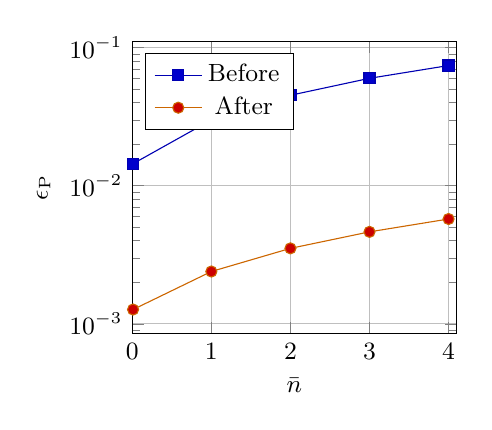
\begin{tikzpicture}
\begin{semilogyaxis}[
 width=0.47\textwidth,height=5.3cm,
 xlabel={$\bar n$},ylabel={$\epsilon_{\rm P}$},
 xmin=0,xmax=4.1,xtick={0,1,2,3,4},
 grid=major,
 legend style={font=\small,at={(0.04,0.96)},anchor=north west},
 tick label style={font=\small},label style={font=\small}]
\addplot+[mark=square*,blue!70!black] coordinates {
(0.01,0.01443531683)
(1,0.02993288433)
(2,0.04515101078)
(3,0.05988834794)
(4,0.07411102521)
};
\addlegendentry{Before}
\addplot+[mark=*,orange!80!black] coordinates {
(0.01,0.001271304448)
(1,0.002394762198)
(2,0.003522057976)
(3,0.00463731733)
(4,0.005744329701)
};
\addlegendentry{After}
\end{semilogyaxis}
\end{tikzpicture}
\hfill
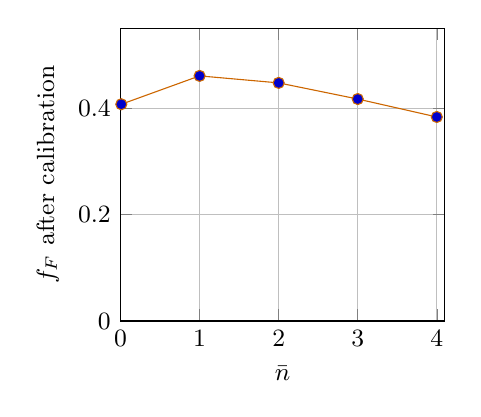
\begin{tikzpicture}
\begin{axis}[
 width=0.47\textwidth,height=5.3cm,
 xlabel={$\bar n$},ylabel={$f_F$ after calibration},
 xmin=0,xmax=4.1,ymin=0,ymax=0.55,xtick={0,1,2,3,4},
 grid=major,tick label style={font=\small},label style={font=\small}]
\addplot+[mark=*,orange!80!black] coordinates {
(0.01,0.4071673042)
(1,0.4604667769)
(2,0.4473048487)
(3,0.4169795052)
(4,0.383271813)
};
\end{axis}
\end{tikzpicture}
\caption{Error of the Pauli approximation. Left: the half-diamond
distance between the reconstructed channel and its Pauli twirl before
and after amplitude calibration. Right: the calibrated discrepancy
in Frobenius norm, normalized to $\|R-I\|_F$. Lines connect the five
sampled points as a visual guide. SDP gaps for the saved matrices
are below $1.1\times10^{-8}$; these gaps do not include uncertainty
from dynamical integration or oscillator truncation.}
\label{fig:distance}
\end{figure}

The normalized Frobenius discrepancy $f_F$ remains between $0.383$
and $0.460$ after calibration. This normalization compares the omitted
channel structure with the residual deviation from the identity.
It is not an error probability or a fraction of the gate infidelity.
The absolute diamond distance and this relative matrix diagnostic
therefore answer different questions. In both cases, the reference
is the Pauli twirl of the same calibrated channel, so the difference
is entirely due to structure discarded by that approximation.

\subsection{The residual discrepancy is concentrated in a collective cross term}
\label{subsec:dominant_component}

The calibrated process matrices contain prominent real entries in
the $(IX,XI)$ and $(II,XX)$ pairs. Their signs and magnitudes satisfy
\begin{equation}
 \operatorname{Re}\chi_{IX,XI}\simeq
 -\operatorname{Re}\chi_{II,XX}=w.
\end{equation}
Including the Hermitian-conjugate entries, this pattern represents
the trace-annihilating map
\begin{align}
 \Delta_{\rm col}(\rho)
 &=w\left(IX\rho XI+XI\rho IX-XX\rho-\rho XX\right)\nonumber\\
 &=w\,\mathcal C_{IX,XI}(\rho).
 \label{eq:channel_cross_pattern}
\end{align}
It is exactly the cross-term structure appearing in
$\Diss[IX+XI]-\Diss[IX]-\Diss[XI]$. Here $\Delta_{\rm col}$ is a
component of a channel difference, and is not itself a physical channel.

We project the off-diagonal part of $\chi$ onto this real pattern.
In the present normalization its coefficient and squared projection
fraction are
\begin{align}
 w&=\tfrac12\left(\operatorname{Re}\chi_{IX,XI}
                    -\operatorname{Re}\chi_{II,XX}\right),\\
 q_{\rm col}
 &=\frac{4w^2}{\|\chi-\operatorname{diag}\chi\|_F^2}.
 \label{eq:pattern_fraction}
\end{align}
The projection accounts for $96.6$--$98.8\%$ of the squared
off-diagonal Frobenius norm (Table~\ref{tab:pattern}). Since the PTM
and canonical $\chi$ Frobenius norms differ by a fixed factor, the
same fraction describes the corresponding PTM projection.
The residual imaginary $(II,XX)$ entry also remains visible and is
consistent with incomplete suppression of the coherent angle error.

\begin{table}[htbp]
\centering
\caption{Collective cross-term pattern after calibration. $w$ and
$\operatorname{Im}\chi_{II,XX}$ are channel-matrix coefficients.
The last column refers to a squared Frobenius norm, not to a fraction
of diamond distance or infidelity.}
\label{tab:pattern}
\begin{tabular}{rrrr}
\toprule
$\bar n$ & $10^3 w$ & $10^3\operatorname{Im}\chi_{II,XX}$ &
$100q_{\rm col}$\\
\midrule
$0.01$ & $0.535249$ & $0.102157$ & $96.65$\\
$1$ & $1.091774$ & $0.211426$ & $97.79$\\
$2$ & $1.651272$ & $0.309838$ & $98.11$\\
$3$ & $2.206694$ & $0.385583$ & $98.41$\\
$4$ & $2.760562$ & $0.426968$ & $98.76$\\
\bottomrule
\end{tabular}
\end{table}

The generator decomposition provides a complementary consistency
check. At $\bar n=4$ after calibration,
$s_{IX}\simeq s_{XI}\simeq2.820\times10^{-3}$ and
$c_{IX,XI}=2.795\times10^{-3}$ per gate, consistent with a
substantial collective-$X$ contribution. These generator coefficients
are distinct from the finite-channel coefficient $w$. Further
components are present: a three-component generator fit leaves
relative residuals of approximately $27.7\%$ at $\bar n=0.01$ and
$5.0\%$ at $\bar n=4$. The concentration of the \emph{discarded
channel terms} in Eq.~\eqref{eq:channel_cross_pattern} consequently
does not imply that three generator terms describe the entire
noisy channel.

This establishes which matrix pattern dominates the discrepancy in
the stated Frobenius metric. Its microscopic coefficient may receive
contributions from both thermal residual motion and explicit motional
noise. Matched noise-source ablations after calibration are needed
to separate those contributions quantitatively.

\subsection{State-resolved consequences of the discarded terms}

Consider the Bell states
\begin{equation}
 \ket{\Phi^+}=\frac{\ket{00}+\ket{11}}{\sqrt2},\qquad
 \ket{\Psi^-}=\frac{\ket{01}-\ket{10}}{\sqrt2}.
\end{equation}
Both are $XX$ eigenstates, so the ideal MS operation leaves their
density matrices unchanged. Their survival infidelities can therefore
be evaluated directly with the post-gate error channel,
\begin{equation}
 r_\psi(\mathcal E)=1-\bra\psi
           \mathcal E(\ket\psi\bra\psi)\ket\psi.
\end{equation}
The collective cross term in Eq.~\eqref{eq:channel_cross_pattern}
contributes
\begin{equation}
 r_{\Phi^+}(\mathcal E)-r_{\Phi^+}(\mathcal E_{\rm P})\simeq 2w,
 \qquad
 r_{\Psi^-}(\mathcal E)-r_{\Psi^-}(\mathcal E_{\rm P})\simeq-2w.
 \label{eq:bell_difference}
\end{equation}
Re-evaluating the saved matrices at all five occupations verifies
these relations with a maximum absolute residual of
$2.2\times10^{-8}$. This is an algebraic attribution within the saved
channels, not a dynamical-convergence error estimate.

\begin{table}[htbp]
\centering
\caption{Bell-state survival infidelity after calibration at
$\bar n=4$, expressed in percent. The full channel and its Pauli
twirl have the same average gate infidelity, $0.93656\%$.}
\label{tab:bell}
\begin{tabular}{lrr}
\toprule
Input state & Full channel & Pauli twirl\\
\midrule
$\Phi^+$ & $1.20748$ & $0.655367$\\
$\Psi^-$ & $0.103253$ & $0.655367$\\
\bottomrule
\end{tabular}
\end{table}

At $\bar n=4$, the survival-probability discrepancy is approximately
$0.00552115$ for each state, with opposite signs
(Table~\ref{tab:bell}). The Pauli approximation thus underestimates
one state infidelity and overestimates the other. For any state and
any measurement event, the absolute probability discrepancy is
bounded by $\epsilon_{\rm P}$. These Bell-state tests provide a
lower bound that reaches approximately $96.1\%$ of the calculated
diamond distance at this occupation. They give an explicit
operational example of the approximation error without invoking
a particular error-correction code.

\section{Discussion}

The results distinguish the suppression of a calibrated angle error
from the accuracy of a Pauli description of the remaining channel.
In the sampled conditions, amplitude feedback reduces both the
infidelity and the distance to the Pauli twirl. A real cross-term
pattern nevertheless dominates the discarded matrix elements and
produces opposite biases in Bell-state survival probabilities.
Consequently, agreement in average gate fidelity alone does not
validate the Pauli approximation for state-resolved predictions.
An application with a specified probability-error tolerance can
use the channel distance as a bound, while its actual sensitivity
depends on the input and measurement.

The interpretation builds on known MS-gate physics. Collective-spin
Kraus operators have already been obtained for motional dephasing
by Ma \textit{et al.}~\cite{Ma2025}; higher-order coherent errors and
drive corrections are treated by Kirchhoff \textit{et al.}~\cite{Kirchhoff2025}.
The present comparison combines a specified finite-Lamb--Dicke
model, several dissipators, amplitude recalibration, and a direct
assessment of the Pauli replacement. Establishing the quantitative
increment beyond these works requires matching their Hamiltonian
conventions, noise assumptions, and calibration objectives in the
overlapping regime. A difference of parameter values by itself
does not establish that increment.

Several restrictions determine the scope of the result. The effective
Hamiltonian retains only a relative $O(\eta^2)$ correction to one
sideband, uses one motional mode, and omits additional optical
couplings. Dissipative rates, including scattering, are fixed as
the amplitude is changed. Calibration is performed independently
at every temperature and targets $h_{XX}$ within a finite tolerance.
These results therefore describe that protocol and do not establish
the optimum over all experimentally available control choices.

The channel comparison concerns a mathematical approximation to the
original calibrated gate. Implementing randomized Pauli operations
would instead change the physical protocol and requires its own
analysis. Similarly, the diamond distance for one reconstructed
gate does not determine a logical error rate. Circuit predictions
would also require attention to motional memory: an initially
factorized thermal mode is assumed for each channel reconstruction.
These restrictions allow the approximation error to be assessed
at the single-gate level without assigning an untested QEC impact.

\section{Conclusion}

We have evaluated the Pauli approximation to saved two-qubit MS
error channels before and after drive-amplitude calibration.
Calibration substantially reduces the channel discrepancy, while
real collective-$X$ cross terms remain the dominant discarded
structure in Frobenius norm. The same terms account quantitatively
for opposite changes in two Bell-state survival probabilities.
The working result is a channel-level measure and diagnosis of
the residual approximation error in the specified model.
Final propagation convergence and a matched comparison with
existing collective-noise models are needed to establish the
quantitative scope of the manuscript.

\appendix
\section{Author checks before submission}
\label{sec:author_checks}

\draftnote{This appendix is an internal work list and should be removed
or converted into validated supplementary material for submission.}

\begin{enumerate}
\item \textbf{Converge the reported quantities.}
Repeat selected calibrated calculations with larger oscillator
cutoffs, finer Hamiltonian coefficient grids, and tighter ODE
tolerances. Compare $\epsilon_{\rm P}$, $w$, $q_{\rm col}$, and
the Bell-state discrepancies themselves. A small SDP gap is not
a substitute for these checks.
\item \textbf{Compare the closest channel model.}
Match the motional-dephasing-only, leading-Lamb--Dicke limit to
Ref.~\cite{Ma2025}, including spin-axis and coupling conventions,
before comparing the finite-Lamb--Dicke and calibrated cases.
Document which changes reflect an established mechanism and which
extend its quantitative characterization.
\item \textbf{Resolve the physical sources after calibration.}
At fixed calibrated controls, compare full noise, zero explicit
dissipation, and selected motional-noise ablations. Separate this
source attribution from a protocol that recalibrates each ablated
model independently. Check whether remaining Hamiltonian terms
affect the claimed non-Hamiltonian interpretation.
\item \textbf{Audit numerical corrections.}
Report raw-to-CPTP-projected changes for the final observables
and ensure they are smaller than the effects being interpreted.
Keep the stored QuTiP and canonical $\chi$ conventions distinct.
\end{enumerate}

\begin{thebibliography}{99}
\bibitem{MS2000}
A. S{\o}rensen and K. M{\o}lmer,
\emph{Entanglement and quantum computation with ions in thermal motion},
Phys. Rev. A \textbf{62}, 022311 (2000).
\href{https://arxiv.org/abs/quant-ph/0002024}{arXiv:quant-ph/0002024}.

\bibitem{Lotshaw2023}
P. C. Lotshaw \textit{et al.},
\emph{Modelling noise in global M{\o}lmer--S{\o}rensen interactions
applied to quantum approximate optimization},
Phys. Rev. A \textbf{107}, 062406 (2023).
\href{https://arxiv.org/abs/2211.00133}{arXiv:2211.00133}.

\bibitem{Kirchhoff2025}
S. Kirchhoff, F. K. Wilhelm, and F. Motzoi,
\emph{Correction formulas for the M{\o}lmer--S{\o}rensen gate under
strong driving}, PRX Quantum \textbf{6}, 010328 (2025).
\href{https://arxiv.org/abs/2404.17478}{arXiv:2404.17478}.

\bibitem{Tinkey2021}
H. N. Tinkey, A. M. Meier, C. R. Clark, C. M. Seck, and K. R. Brown,
\emph{Quantum process tomography of a M{\o}lmer--S{\o}rensen gate
via a global beam} (2021).
\href{https://arxiv.org/abs/2101.04648}{arXiv:2101.04648}.

\bibitem{Ma2025}
Y. Ma, M. Hanks, E. Gneusheva, and M. S. Kim,
\emph{Reshaping quantum device noise via repetition code circuits},
Phys. Rev. Research \textbf{7}, 033262 (2025).
\href{https://arxiv.org/abs/2411.00751}{arXiv:2411.00751}.

\bibitem{Grossman2026}
O. Grossman \textit{et al.},
\emph{Trapped-Ion Multiqubit Gates are Compatible with Scalable
Quantum Error Correction}, preprint (2026).
\href{https://arxiv.org/abs/2605.28536}{arXiv:2605.28536}.

\bibitem{QPT}
I. L. Chuang and M. A. Nielsen,
\emph{Prescription for experimental determination of the dynamics
of a quantum black box}, J. Mod. Opt. \textbf{44}, 2455--2467 (1997).
\href{https://doi.org/10.1080/09500349708231894}{doi:10.1080/09500349708231894}.

\bibitem{Markovian_Errors}
R. Blume-Kohout \textit{et al.},
\emph{A Taxonomy of Small Markovian Errors},
PRX Quantum \textbf{3}, 020335 (2022).
\href{https://arxiv.org/abs/2103.01928}{arXiv:2103.01928}.

\bibitem{WatrousDiamond}
J. Watrous, \emph{Simpler semidefinite programs for completely bounded
norms} (2012).
\href{https://arxiv.org/abs/1207.5726}{arXiv:1207.5726}.
\end{thebibliography}
\end{document}
